\documentclass[a4paper,10pt]{report}
\usepackage[utf8x]{inputenc}

% Code-Listings
\usepackage{listings,color} 
\lstset{numbers=left, numberstyle=\tiny, numbersep=5pt,basicstyle=\footnotesize,breaklines=true} 
\lstset{language=Java}

% Glossary
\usepackage{nomencl}
\makenomenclature

% Allow Hyperlinks in the PDF
\usepackage{hyperref}  
\hypersetup{colorlinks=false,
            pdftitle={Refactoring Extenstion for the Yeti NesC Eclipse Plugin},
            pdfauthor={Noah Heusser, Max Urech},
            pdfsubject={Documentation of the Refactoring Extenstion for the Yeti NesC Eclipse Plugin},
            pdfkeywords={Refactoring, NesC, Yeti, TinyOS, Eclipse, LTK, Language Toolkit, ETH},
            pdfborder={0 0 0}
} 

% Grafics
\usepackage{graphicx}
\usepackage[dvipdfm]{geometry}

% Title Page
\title{Refactoring Extenstion for the Yeti NesC Eclipse Plugin}
\author{Noah Heusser, Max Urech}


\begin{document}
\maketitle

\begin{abstract}
In todays Software Development Processes agile development is the state of the art. Agile Processes lead to frequent code reorganisations or in one words ``Refactoring''.
Refactoring can be a lot of boring and error-prone work if a Developer has to do it by hand. One can easy see that a Computer is mutch faster and far more reliable if
it comes to finding all occures of a Variable name and change them to a new name.

A Refactoring Plugin like the one we wrote allows the Software Developer to concentrate on the Design of the Software and let the computer do the busy work. This Document
discribes the used Frameworks and explains the Solution we developed.

After all today we have a working Refactoing Plugin which allows to rename most Elements of the NesC language. We could also introduce some other Refactorings like 
``Introduce Alias'' or ``Extract Function'', but in this area a work could still be done.

We hope you enjoy using our Software and also the reading of this Document. 
\end{abstract}

\tableofcontents

\part{What is refactoring}
\chapter{Definition of refactoring}
Wikipedia gives us the following definition for code refactoring:
``Code refactoring is the process of changing a computer program's source code without modifying its external functional behavior in order to improve some of the nonfunctional attributes of the software. 
Advantages include improved code readability  and reduced complexity to improve the maintainability of the source code, as well as a more expressive internal architecture or object model to improve extensibility.''
Since this document is about a refactoring facility for NesC, we are of course actually always referring to code refactoring, when we talk about refactoring.

\chapter{Why do we need refactoring}
Reusability and maintainability are two terms, which are known to everybody, who ever heard something about software engineering. 
A refactoring facility is a means for supporting those properties. I.e. if you want to reuse an existing function in a program in a second place,
you might suddenly realise, that the name of the function actually not really matches its purpose and you consequently want to rename it to a more appropriate name.
If you have a function rename refactoring at hand at this point, you simply have to select the refactoring, type in the name, press enter and you are done. 
Without such a tool you had to replace the function name by hand at every position in the program, where it appears, possibly in different files.
This example is also good for the cast, that refactoring supports maintainability, because a readable program is also a maintainable program. 
And if the names of the different entities in a program match their purpose, the program is for sure more readable, then if they don't.

\part{Eclipse Plugins}
\chapter{General Infos about writeing Plugins}
Eclipse is famous for it's plugin architecture. Everything in Eclipse is a Plugin. An Eclipse Plugin is a JAR-File or a Folder in the plugins-Directory of the eclipse program folder.
To be a plugin it takes at least three Files.
\begin{itemize}
  \item META-INF/MANIFEST.MF
  \item plugin.xml
  \item plugin.class
\end{itemize}

\section{META-INF/MANIFEST.MF}
The Manifest file is the first File that is read by Eclipse while loding the Plugin. It conatins all the Informations about what requirements 
are needed to load the Plugin and how it can be loaded. I will now explain the most important entrys in the Manifest file.

\begin{lstlisting}[caption=MANIFEST]{META-INF/MANIFEST.MF}
Manifest-Version: 1.0
Bundle-ManifestVersion: 2
Bundle-Name: TinyOS_Refactoring
Bundle-SymbolicName: tinyos.yeti.refactoring;singleton:=true
Bundle-Version: 1.0.0
Bundle-Activator: tinyos.yeti.refactoring.RefactoringPlugin
Require-Bundle: org.eclipse.ui,
 org.eclipse.core.runtime,
 tinyos.yeti.core;bundle-version="2.2.17",
 tinyos.yeti.parser.nesc12;bundle-version="1.2.17",
 org.eclipse.ui.workbench.texteditor;bundle-version="3.5.1",
 org.eclipse.ltk.core.refactoring;bundle-version="3.5.0",
 org.eclipse.ltk.ui.refactoring;bundle-version="3.4.101",
 org.eclipse.core.resources;bundle-version="3.5.2",
 org.eclipse.jface.text;bundle-version="3.5.2",
 org.eclipse.ui.ide;bundle-version="3.5.2",
 org.eclipse.ui.editors;bundle-version="3.5.0",
 tinyos.yeti.preprocessor.nesc12;bundle-version="1.2.17",
 org.eclipse.core.expressions;bundle-version="3.4.101"
Bundle-ActivationPolicy: lazy
Bundle-RequiredExecutionEnvironment: JavaSE-1.6
\end{lstlisting}


\begin{description}
 \item[Manifest-Version] This line shows that a manifest's entries take the form of "header: value" pairs. The name of a header is separated from its value by a colon. (from http://java.sun.com/developer/Books/javaprogramming/JAR/basics/manifest.html access 2.9.2010)
 \item[Bundle-ManifestVersion] Manifest header identifying the bundle manifest version. A bundle manifest may express the version of the syntax in which it is written by specifying a bundle manifest version. Bundles exploiting OSGi Release 4, or later, syntax must specify a bundle manifest version. 
The bundle manifest version defined by OSGi Release 4 or, more specifically, by version 1.3 of the OSGi Core Specification is "2". (from Eclipse Help Version: 3.5.2)
 \item[Bundle-Name] A human readable meaningful Name for the Plugin you write.
 \item[Bundle-SymbolicName] A unique String identifyer for you Pulugin. Mostly the Path of your package structure is used. The \verb!singelton:=true! makes the OSGi Framework only load your Plugin once. It has to be set in every Eclipse Plugin. It is only necessary cause Eclipse uses OSGi which is not only used for Eclipse.
 \item[Bundle-Version] Defines the Version of the Plugin. When the Plugin is used by an other Plugin , it can specify the Verserion in the Required-Bundle Parmeter. A Verstion is composed of 3 positive natural numbers and a String seperated by ``.'' sign. Two Versions are equal if the Numbers are Equal. The String in the end might be used to specify different Versions with the absolute same Interface (for example different Compailers). The Nummbers from left to right are called: Major.Minor.Mirco.
 \item[Bundle-Activator] This is the Path of the Class which is used to start the whole Plugin. The class must extend \verb!org.eclipse.core.runtime.Plugin!. 
 \item[Require-Bundle] When you write you plugin you will use the Functionality of other Plugins. To do that you have to specify here which plugins you use. Eclipse will refuse to load your plugin if the Plugins you require are not avialable. In addition you can specify the version of the plugin you need to be available. If you don't specify anything else Eclipse will assume to have an compatible Version as long as there is one having the same Major-Number. In case of you have to be more picky, you can also add a \verb!match! parameter with \verb!perfect! for Major, Minor and Micro Number have to match, or \verb!equivalent! for Major and Minor Number have to match.
 \item[Bundle-ActivationPolicy] The only parameter you can add here is \verb!lazy! which tells OSGi to wait with loading the Plugin until it is used.
 \item[Bundle-RequiredExecutionEnvironment] Defines a lower bound for the Version of the JVM that is allowed to be used.
 \end{description}

\section{plugin.xml}
The {\it plugin.xml} file was once reponsable for all the things that are now configured in the {\it MANIFEST.MF} File. If you search the Internet you will have problems to find what you want cause of that. Today the {\it plugin.xml} is responsable for offering and using Extention Points. I will not talk about how to offer an Extenstion point, cause for this Project it wasnt necessary.

\subsection{Using Extenstion Points (making Extenstions)}
When you want to use an Extenstion Point, you have to add the Plugin which defines the Extenstion Point to you Require-Bundle list in the {\it MANIFEST.MF}. Mostly you will have found the Extenstion Point you want to use by Google and often you don't know what Plugin is offering that Extention Point. The only advice I can give you is to use Google again or grep throu the plugins Directory of Eclipse. We did not find a way in which one could easely find the right Plugin.

When the right Plugins are included, one can use the Extenstion Points by adding a \verb!<extension>! Tag.
\begin{lstlisting}[language=XML,caption=Use Extenstion Point ({\it plugin.xml})]{plugin.xml}
<?xml version="1.0" encoding="UTF-8"?>
<?eclipse version="3.4"?>
<plugin>
 	<extension 
	    point="org.eclipse.core.expressions.propertyTesters">
   		<propertyTester ... />
 	</extension>
</plugin>
\end{lstlisting}

The \verb!<extenstion>! Tag has only one Important Attribute. It is the Extenstion Point you want to use. In this case of our Example we use the Extenstion Point \verb!propertyTesters! form the Plugin \verb!org.eclipse.core.expressions!.

The Tags between \verb!<extension>! and \verb!</extension>! are informations for the Extention Point. What Tags need to be there can be read in the XML-Schema File in the \verb!org.eclipse.core.expressions! Plugin Jar. I won't go into detail here, but the plugin.xml of the Plugin that provides the Extention Point defines where in the Jar the Schema File is. Eclipse can show the Schema File by clicking on \verb!Show extension point description! in the \verb!Extention!-Tab of the {\it plugin.xml} editor.

Important is to understand how Eclipse calls your Code. First you find the Extenstion Point you want to extend. Then you wirte your XML Code to extend it. For some Extenstion Points a Class, implementing an Interface has to be passed as Attribute. If so the Extenstion Point Loads your Class and executes a Method of that Inferface.


\chapter{Language Toolkit for Processor Based Refactoring}
\label{languageToolkitForProcessorBasedRefactoring}
For our refactoring Plugin we used the Processor based refactoring, offered by the Language Toolkit of Eclipse. I will explain now how such a refactoring works.
\section{Important Classes}

\begin{figure}[h]
\centering
\includegraphics[width=\textwidth]{classDiagrammProcessorBasedRefactoring.png}
\end{figure}

In the class diagramm the most important Classes are shown. While writing Refactorings you won't have to care about the Classes \verb!RefactoringWizardOpenOperation!, \verb!Refactoring! and \verb!ProcessorBasedRefactoring!. This 
classes can be used as they are. All the other Classes need to be extended.
\begin{description}
 \item[RefactoringWizard] When the User starts a Refactoring he is asked for additional Informations. This Form is painted by the \verb!RefactoringWizard! class.
The Connection to the Info class is necessary to store the Informations the user typed into the Form. 
 \item[RefactoringInfo] The \verb!RefactoringInfo! class is not a Class of the LTK Framework, we introduced it to allow communication between the \verb!RefactoringProcessor! and the \verb!RefactoringWizard!. 
The idea to do it that way is from the Article \href{http://www.eclipse.org/articles/Article-LTK/ltk.html}. When writing Refactorings for our Project, you can extend the 
RefactoringInfo class. It supports already some Util functionality.
 \item[RefactoringProcessor] This Class does the actual Refactoring. 
\begin{description}
 \item[isApplicable()] This method checks if the Refactoring can be used. It can be used to enable or disable Menu entrys. Douring my work with the Refactoring Processor, this 
method got never called by the Framework. It can easely be implemented by calling \verb!checkInitialConditions()!.
\begin{lstlisting}[caption=Generic isApplicable Implementation]{PropertyTester.java}
public boolean isApplicable() throws CoreException {
  return checkInitialConditions(new NullProgressMonitor()).
           hasFatalError();
}
\end{lstlisting}
\item[identifyer] Is a unique Identifier for the Processor.
\item[name] A human readable Name for what the Refactoring does.
\item[checkInitialConditions] Checks whether the Refactoring is applicable before the User gives any informations about how the Refactoring should happen. Mostly we checked
here if the User did a valid selection. Cause of the conditionaly visibility we used, it was used to descide whether a Refectoring is offered or not.
The Return value is a Status. If the Refactoring can not be executed, the status must contain fatal Errors. Otherwise the Refactoring is ment to be executable.
\item[checkFinalConditions] Checks whether the Informations the User gave to configure the Refactoring are valid. 
\item[createChange] This is the Method where the Magic happens. All the changes of your Refactoring are made within this Method. The return value is a \verb!Change!. A \verb!Change!
discribes what you want to change in your Refactoring. You don't execute the change yourself, this is done by the Framework. LTK offers a lot of Implementations of the Change
class. 
\end{description}
\end{description}

\section{The Change Classes}
The LTK offers the Change Class. By createing Change Classes in stead of doing the Changes yourself you allow LTK to provied ``change priview functionality'' and ``undo redo''.
LTK offers a lot of Changes for Moving, Renameing and so fonth. I just talk about the most important ones.
\begin{figure}[h]
\centering
\includegraphics[width=\textwidth]{changeClassDiagramm.png}
\end{figure}
\begin{description}
 \item[CompositeChange] Most Refactoings change more than one thing. Thatsway you will use this Change in almost every Refactoring.
 \item[NullChange] A Change that does nothing. It allows you to avoid null-Values within your Code.
 \item[DocumentChange] Changes a TextFile which is opend in the Editor. It allows you to change code that has not yet been saved. We wanted to use this, but got 
Exceptions cause Threads tryed to access Data that are not allowed to access. In the Internet I found People having the same Problem, but no solution. The Problem seems
to occure only in the newest Version of Eclipse. Maybe it is solved when you read that. If so, use this Change for Files that are opend, and not \verb!TextFileChange!.
 \item[TextFileChange] We used the \verb!TextFileChage! to do all our TextChanges. It works, but the User is forced to save all Files before he can start doing 
Refactoring. 
\end{description}



\section{Refactoring Operation Sequence}
Now you know all the Classes. I will no outline what happen when a Refactoring takes place. 
\begin{figure}[h]
\centering
\includegraphics[width=\textwidth]{interactionDiagramRefactoring.png}
\end{figure}
First, (not in the Picture) the User starts a Refactoring by clicking on a menu entry. The \verb!ActionHandler! gets called and initializes all necessary classes.
You can see that the \verb!RefactoringWizard! and the \verb!RefactoringProcessor! bouth get a link to the \verb!Info! Object. If you are working with the Selection, 
the Selection to the \verb!Info! Object in the ActionHandler, later it is hard, cause you are in the wrong thread.

Then the \verb!ActionHandler! calls the \verb!run()! Method of the \verb!RefactoringWizardOpenOperation!. I have to say that the Calls which are done by the
\verb!RefactoringWizardOpenOperation! are not realy done by the \verb!RefactoringWizardOpenOperation! Class. But it would become very complex to explain how it realy works.
The effect you see when your methods are called is as in the Picture.

The \verb!RefactoringWizardOpenOperation! checks if the initialConditions are OK. If not it would show the Status Error Message to the User and terminate. If there
are no Fatal Errors, the \verb!RefactoringWizard! is called to draw the form and save the necessary Informations of the Users to the \verb!Info! Object.

Now, the final Conditions an be checked by the \verb!RefactoringProcessor!. If they are not OK, the Status Errors will be shown to the User and the \verb!RefactoringWizard!
will be shown again. If thay are OK, the \verb!createChange()! method of the \verb!RefactoringProcesser! gets called. A Priview of the Changes is shown to the User.

If the User accepts the Changes, they get applied and the Refactoring is finished. Douring the whole Process, LTK makes shure that the User has \verb!back! and \verb!cancel! Buttons.

\chapter{Menu's with conditional visibility}
\label{menuWithConditionalVisibility}
In our Plugin the Use Case is always the same. The User selects some code, the User selects a refactoring, the User executes the Refactoring. To achieve that we need to have Menus where the user can select the Refactoring he wants to Execute.
But this is not enogh, our Plugin supports a lot of Refactorings. If the User has to find the Refactoring he wants to use in a list of all possible Refactorings, it will take him a lot of time.
To make it easy for the User we want to list only those Refactorings that are actually possible for his momentary Selection. This means we need conditional visibility.

In the picture the necessary components for a Menu with conditional visibility are shown. Dooring the following sections I will explain every component in the Picture.
\begin{figure}[h]
\centering
\includegraphics[width=\textwidth]{menuStructure.png}
\end{figure}

\section{Create a Menu entry}
Eclipse knows about a hundred ways to create a new Menu Entry. Almost none of them make it necessary to write Java, but all of them have different possibilitys. 
Douring our Project we were not able to understand what ways outdated or what the todays state of the art way is. After testing three ways which did not fit our needs,
we chose the one I will explain now. 

\subsection{Add a new Submenu}
We want our Refactoring functionality to be available in two Menus. In the Main Menu of the Eclipse window and the Context menu which appears when one rightclicks on
a selection. To do that we used the \verb!org.eclipse.ui.menus! Extension Point. In this Extenstion Point every menu can be identified by a URI. The URI of the Main Menu is:
\verb!menu:org.eclipse.ui.main.menu! and to define it's Position we add \verb!?after=additions! to the URI. This adds the Menu just after the menus of the additions group, 
which is the core Functionality of the Eclipse IDE. In the UML this \verb!<menu>! Tag is the \verb!MenuContributionMenu! Class.

In XML Code it looks like this:
\begin{lstlisting}[language=XML,caption=Create Menu Folder ({\it plugin.xml})]{plugin.xml}
<extension id="add.item" point="org.eclipse.ui.menus">
  <-- Entrys in the Top Menu -->
  <menuContribution
     locationURI= "menu:org.eclipse.ui.main.menu?after=additions">
    <menu id="tinyos.yeti.RefactoringMenu"
          label="Refactoring" />
  </menuContribution>
</extenstion>
\end{lstlisting}
Important is to see that we use the Tag \verb!<menu>! which means that we add a submenu and that the id of the new Submenu is \verb!tinyos.yeti.RefactoringMenu!. 
Later when we add Commands to that Submenu we have to refer to that id.

To add the Submenu also to the Context menu we add the same XML Block again, but use the URI \verb!popup:org.eclipse.ui.popup.any! and give it the Id \verb!tinyos.yeti.RefactoringPopup!.

If you would now start Eclipse with that new Menu, you wouldnt see anything. The Submenus are only displayed if the Submenu has entrys.
\subsection{Add a Command to the Submenu}
Adding a Command (an Entry which triggers an Action) is also added by the Tag \verb!<menuContribution>! but this time not with the Child-Tag \verb!<menu>! but \verb!<command>!.
In the UML Diagramm I called it \verb!MenuContributionCommand!. For now we don't look at the \verb!visibleWhen!, it will be explanied later.

The \verb!<command>! Tag has three attributes. \verb!lable! is the String the user will see in the Menu. \verb!id! is just a unique identifyer and \verb!commandId! is the 
id of the Command that shell be executed when the user clicks on this entry. Createing that command will be explaind in the next Section.

In XML it looks like this:
\begin{lstlisting}[language=XML,caption=Adding a Command to Menu ({\it plugin.xml})]{plugin.xml}
<extension id="add.item" point="org.eclipse.ui.menus">
  <menuContribution
       locationURI= "menu:tinyos.yeti.RefactoringMenu?after=additions">
    <command commandId="tinyos.yeti.refactoring.rename.local.variable"
             id= "RenameLocalVariable"
             label= "Rename Local Variable" />
  </menuContribution>
</extension>
\end{lstlisting}
You can see that the \verb!menuContribution! goes this time to \verb!tinyos.yeti.RefactoringMenu! which we defined in the last section.

\subsection{Createing a Command}
This is now the Command that is called Command in the UML Diagramm. It is not in the Extenstion Point \verb!org.eclipse.ui.menus! but in the Extenstion Point \verb!org.eclipse.ui.commands!. 
The \verb!<command>! Tag has three attributes. An \verb!id! which is a unique Identifiere. The \verb!categoryId! which groups the the \verb!<command>!'s to Categroies.
We never used the Categories so we just introduced one and gave all our commands this Category. We hoped that it would be possible to fill a Submenu with a Category of Commands.
But we didn't find a way to do that. The third Parameter is a \verb!name!. We never used it eather, we usualy took the label in the Menu also as name of the Command.

In XML it looks like this:
\begin{lstlisting}[language=XML,caption=Createing a Command ({\it plugin.xml})]{plugin.xml}
<extension point="org.eclipse.ui.commands">
  <category id="tinyos.yeti.refactoring"
            name="Refactoring" />
  <command id="tinyos.yeti.refactoring.rename.local.variable"
           categoryId="tinyos.yeti.refactoring"
           name="Rename Local Variable"/>
</extension>
\end{lstlisting}

One can ask now, where does Eclipse know from what Method it has to invoke to call that command. Well it does not. To know that, we have to define a \verb!handel!.

\subsection{Intoducing a Handler for a Command}
A handler is connects a Command in the XML File to a Java Class which implement the Interface \verb!org.eclipse.core.commands.IHandler!. The Extenstion Point
\verb!org.eclipse.ui.handlers! helps doing that job. It is very simple. Just the Class and the \verb!commandId!.
\begin{lstlisting}[language=XML,caption=Connecting a Command to a Handler ({\it plugin.xml})]{plugin.xml}
<extension point="org.eclipse.ui.handlers">
   <handler class="tinyos.yeti.refactoring.entities.variable.rename.local.RenameLocalVariableActionHandler"
            commandId="tinyos.yeti.refactoring.rename.local.variable" />
</extention>
\end{lstlisting}

\subsection{Bindings}
We did not yet speak about Bindings. They allow you to introduce Shortcuts for your Commands. We did it first, but removed it later again.
I think the following Code explains itself:
\begin{lstlisting}[language=XML,caption=Introduce Shortcuts ({\it plugin.xml})]{plugin.xml}
<extension point="org.eclipse.ui.bindings">
                <!--
                        One could also add a Shortcut, by adding the following Attribute
                        to the <key>-Tag,
                        for example: sequence="M1+M2+r"

                        The M Keys in the sequence are Platform independent keys.
                                On PCs they are mapped to:
                M1 = Ctrl
                M2 = Shift
                M3 = Alt

                The upper example would the the shortcut: Ctrl+Shift+r
		-->
                <key commandId="tinyos.yeti.refactoring.rename.local.variable"
                     schemeId="org.eclipse.ui.defaultAcceleratorConfiguration"
                     sequence="M1+M2+r" />
</extenstion>
\end{lstlisting}

\section{Add conditional visibility}
Up to now all our menu entrys will allways be available no matter whether the User did a valid selection or not. But in the beginning of this Chapter we desided to show only 
those Refactorings that are executable for the momentary selection.
\subsection{Property Tester}
To do that we use the Extenstion Point \verb!org.eclipse.core.expressions.propertyTesters!. It allows to define a \verb!propertyTester! with a list of Propertys. In our
case we defined one \verb!propertyTester! called \verb!tinyos.yeti.refactoring.AvailabilityTester! which has one property for each Refactoring.

In XML:
\begin{lstlisting}[language=XML,caption=Property Tester ({\it plugin.xml})]{plugin.xml}
<extension point="org.eclipse.core.expressions.propertyTesters">
  <propertyTester id="tinyos.yeti.refactoring.AvailabilityTester"
                  type="org.eclipse.jface.text.ITextSelection"
                  namespace="tinyos.yeti.refactoring.isAvailable"
                  properties="renameLocalVariable, ..."
                  class="tinyos.yeti.refactoring.AvailabilityTester" />
</extension>
\end{lstlisting}

One can see that is has a \verb!class! Parameter. This is a Java Class that extends \verb!org.eclipse.core.expressions.PropertyTester!. It has only one abstract Method:
\begin{lstlisting}[caption=extends PropertyTester]{PropertyTester.java}
public class AvailabilityTester extends PropertyTester {

  public boolean test(Object receiver, String property, Object[] args,Object expectedValue) {
    
  }
}
\end{lstlisting}
One can see that there is a String \verb!property!. It is exactly the String that is defined in the \verb!property! Attribute of the \verb!propertyTester! Tag.
This way we wrote for each Refactoring a Test wether it is available or not.

\subsection{Visibility Condition}


\begin{lstlisting}[language=XML,caption=Visibility Condition ({\it plugin.xml})]{plugin.xml}
<extension id="add.item"
           point="org.eclipse.ui.menus">
  <menuContribution locationURI= "menu:tinyos.yeti.RefactoringMenu?after=additions">
    <command commandId="tinyos.yeti.refactoring.rename.local.variable"
             id= "RenameLocalVariable"
             label= "Rename Local Variable">
      <visibleWhen checkEnabled="false">
        <iterate ifEmpty="false">
          <!-- The forcePluginActivation-Parameter is absolutly necessary. 
               Otherwise the Property gets never checkt -->
          <test property="tinyos.yeti.refactoring.isAvailable.renameLocalVariable"
                forcePluginActivation="true" />
        </iterate>
      </visibleWhen>
    </command>
  </menuContribution>
</extenstion>
\end{lstlisting}
In the MenuContributionCommand we add a \verb!visibleWhen! Tag. The \verb!checkEnabled="false"! disables the check whether the Command is available or not. 
It is a Functionality provided by the Handler Class. Technicaly it would work whith just writing \verb!checkEnabled="true"! and Implementing the functionality in 
the ActionHandler. But as the name isEnabled sais, it is not the Idea of this Function. Thatsway we prefered doing it with the Property.

The \verb!visibleWhen! is necessary cause it seems to be a collection that we get there. If it is not there it wont work.

\part{The Refactoring Plugin}
\chapter{About our plugin}
The refactoring plugin is an extension for the Eclipse Yeti plugin. Its target is to accelerate the development of NesC code and make it more convenient.
This is achieved by automating low level, time consuming tasks.
\section{The general refactoring life cycle}
From a user perspective the general refactoring life cycle looks like this:
   \begin{enumerate}
     \item The user selects a new text range in his nesc editor.
     \item Eclipse instantiates a {\it RefactoringAvailabilityTester} class, which is a subtype of the {\it PropertyTester} class, which is defined by Eclipse.
     \item Eclipse checks all refactorings defined in the {\it plugin.xml} against the property tester, and memorises which of them are available. 
     \item Eclipse shows the available refactorings in the top menu bar, as well as in the popup menu.
     \item The user selects a refactoring, which he wants to execute.
     \item Eclipse will execute the appropriate action handler.
     \item The user probably has to do some input.
     \item Eclipse shows the changes to be done in a preview window.
     \item The user confirms or denies the changes.
     \item Eclipse finishes the refactoring.
   \end{enumerate}
This life cycle can be divided in two main parts. The first part is the evaluation of the available refactorings and the second part is the actual execution of a specific refactoring. 
This partitioning has two major advantages. First it allows a better user experience, since he sees only the refactorings, which are really executable for the current selection. 
Second, the execution of a refactoring does not have to care, if the refactoring is applicable.\\
In the graphic on page \pageref{UserInputSequence} you can see the steps the user has to take in order to execute a refactoring.

\newpage
\begin{figure}[h]
\centering
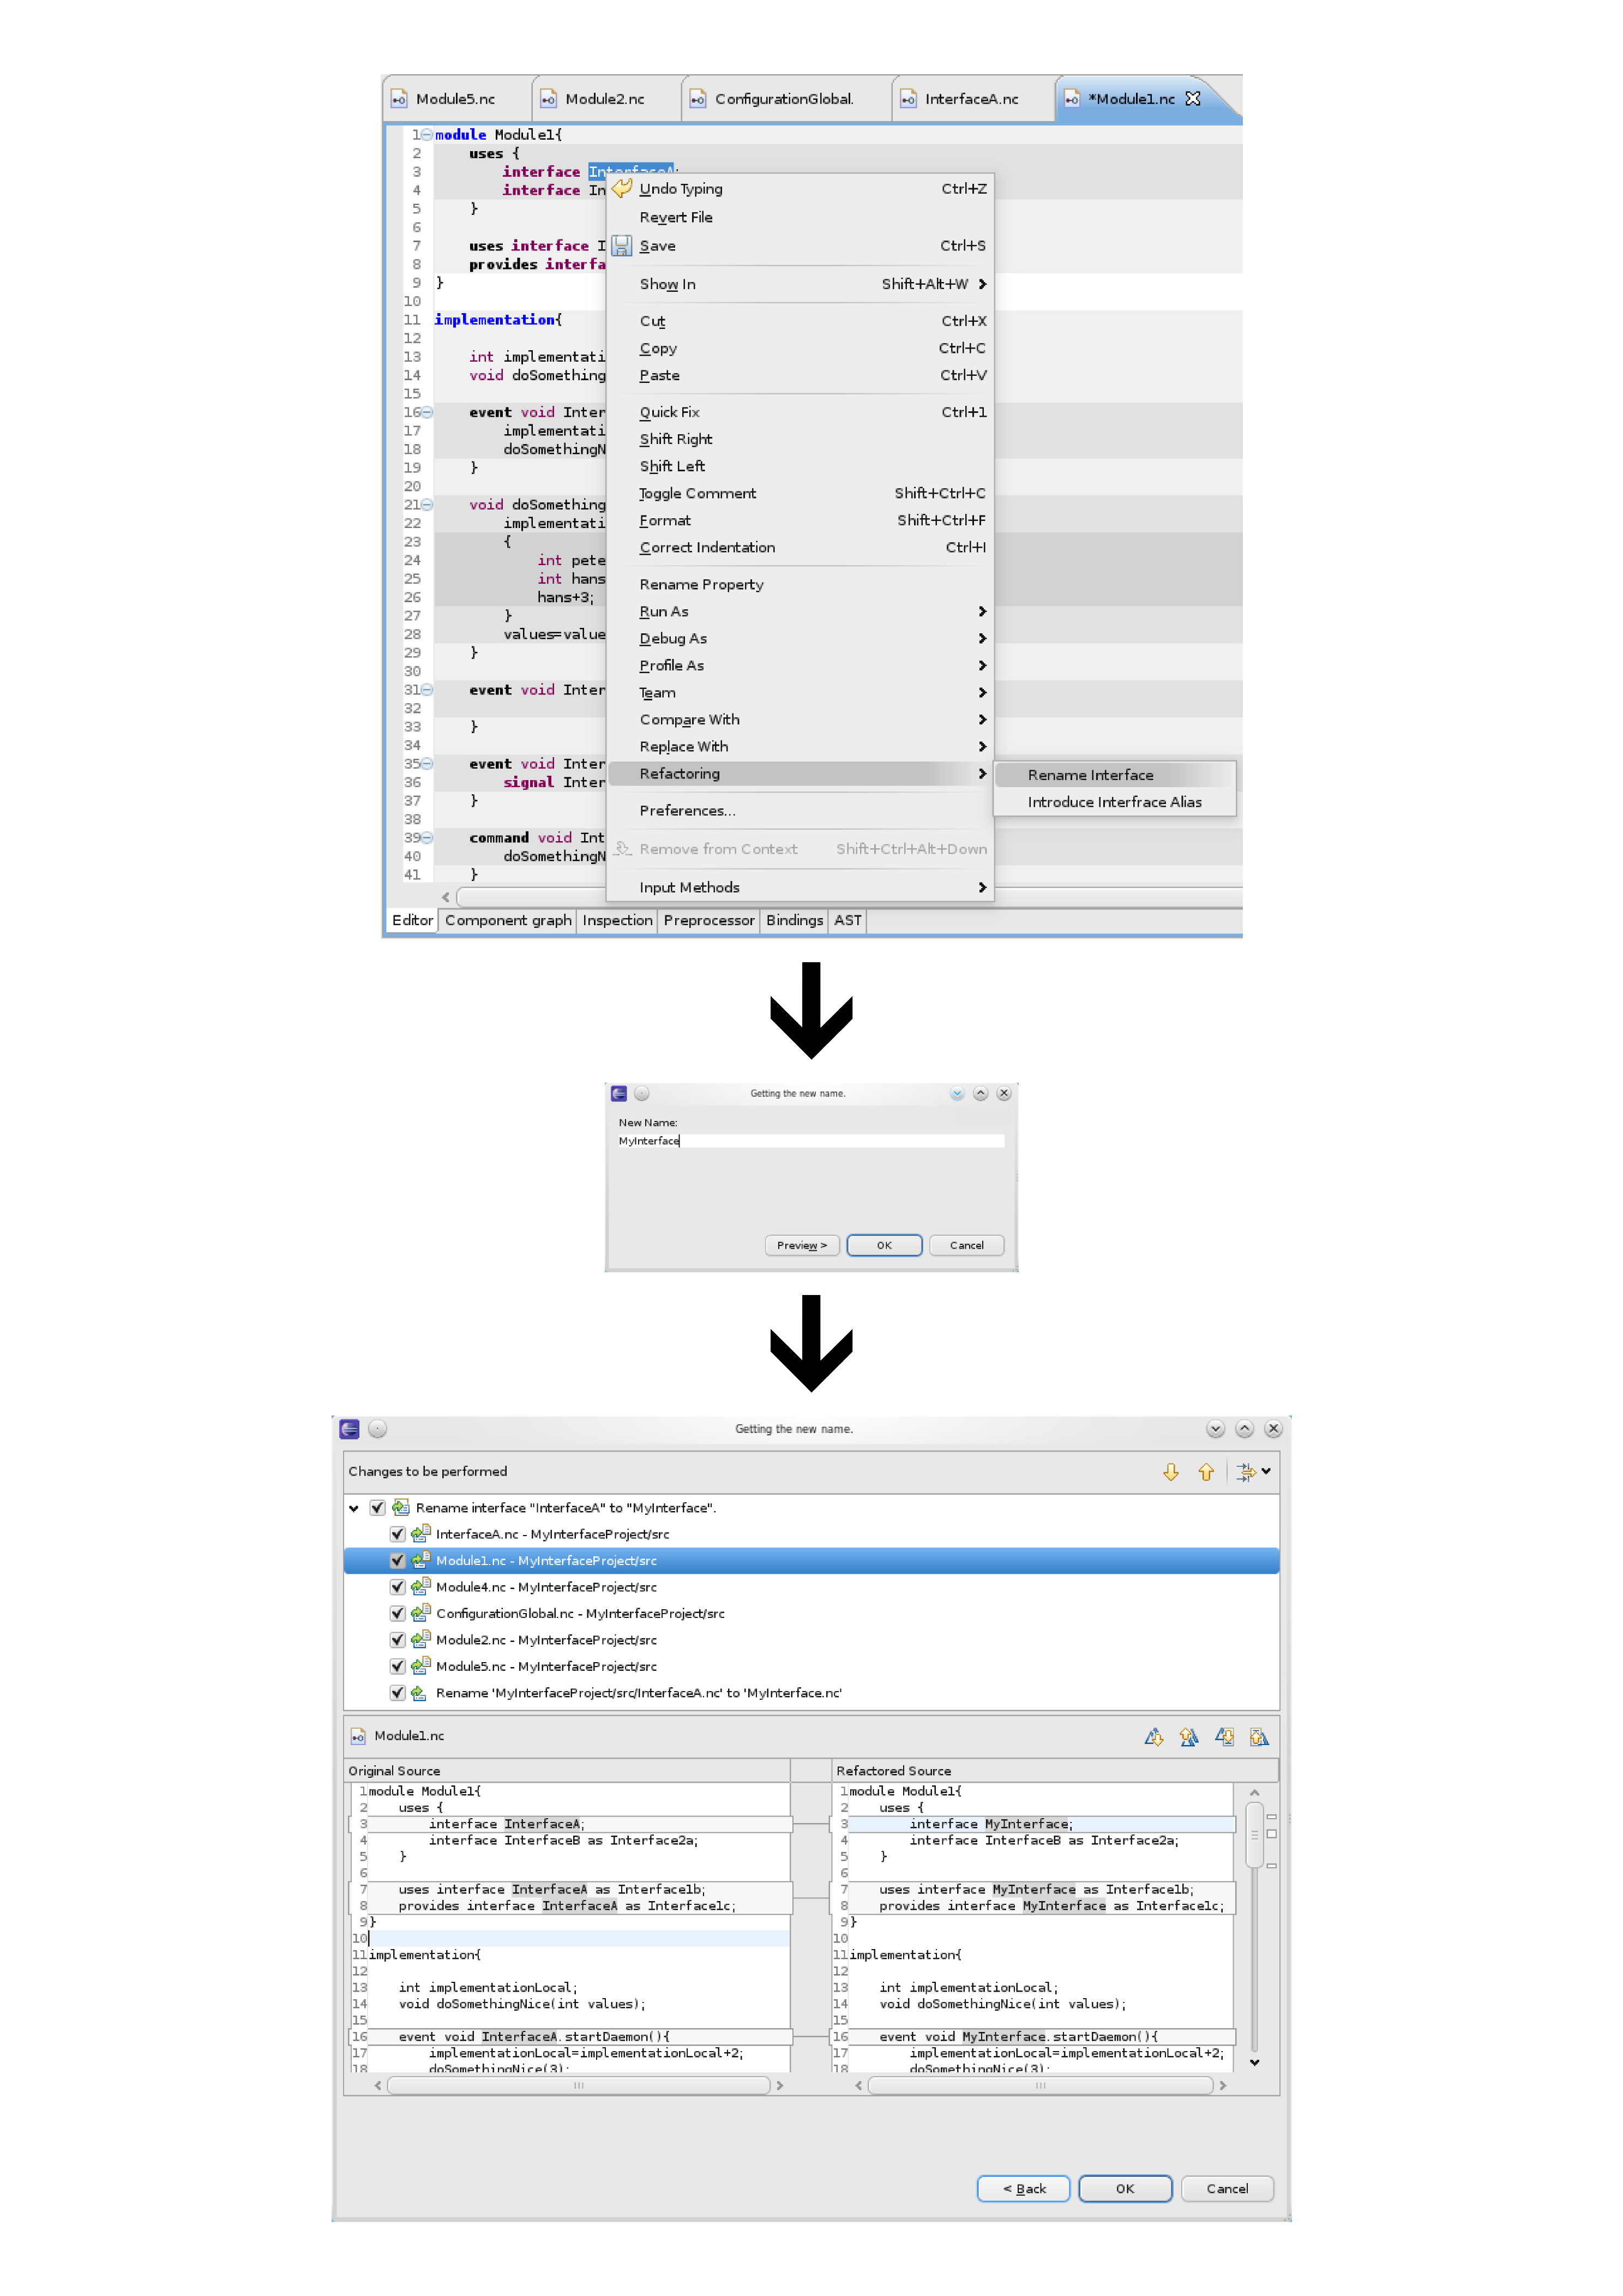
\includegraphics[height=0.98\textheight]{userInputSequence.png}
\caption{A standard user interaction with the refactoring plugin.}
\label{UserInputSequence}
\end{figure}

\section{Package structure}
The root package of the plugin is {\it tinyos.yeti.refactoring}. It contains the {\it RefactoringPlugin} class, which is required for an Eclipse plugin, as well as the classes we gone talk about in the chapter "From plugin XML to java code".\\
The root package contains four subpackages:
   \begin{enumerate}
     \item The {\it abstractrefactorings} package
     \item The {\it ast} package
     \item The {\it utilities} package
     \item The {\it entities} package
   \end{enumerate}
The {\it abstractrefactorings} package contains infrastructure classes, used to implement concrete refactorings. We take a closer look at this classes in the "Abstract refactorings" chapter.\\
The {\it ast} and {\it utilities} packages include classes, which are used to interact with the AST and the project, in which we are doing refactoring. The contents of this packages are explained in the chapter "Harnessing the AST".\\
The {\it entities} package is actually the root package for all concrete refactoring implementations. By entity we mean an object which can be modified by a refactoring. I.e. the entity of a rename or extract function refactoring is a function. The entity of a rename or introduce interface alias is an interface alias.
Therefore the next level of packages in the {\it entities} package will designate a entity, and the package in such a specific package will designate a concrete refactoring. This means that you will find the concrete implementation of the rename interface alias refactoring implementation in the subpackage {\it entities.interfaces.alias.rename}.
About concrete refactorings we will talk in the chapter "Concrete refactorings".


\chapter{From plugin XML to Java code}
\label{fromPluginXMLToJavaCode}
\section{How to decide the availability of a refactoring}
After we have introduced the appropriate lines of XML in the {\it plugin.xml} for a specific refactoring, the plugin is now able to ask the question: ``Is the current selection appropriate for this refactoring?''
But the software is not yet capable to answer this question. That is where the {\it Refactoring} enum and the {\it RefactoringAvailabilityTester} come in. 
An overview of the relations described in this chapter is given in the graphic on page \pageref{AvailabilityTesterContext}.

\begin{figure}[h]
\centering
\includegraphics[height=.5\textheight]{AvailabilityTesterContext.png}
\caption{The {\it RefactoringAvailabilityTester} class and its context}
\label{AvailabilityTesterContext}
\end{figure}

\subsection{The {\it Refactoring} enum}
The {\it Refactoring} enum defines for each refactoring, which is defined in the {\it plugin.xml}, its corresponding counterpart in java code as an enum constant.
Every such enum constant has three fields:
   \begin{enumerate}
     \item {\it propertyName} of type {\it String}
     \item {\it entityName} of type {\it String}
     \item {\it tester}  of type {\it IRefactoringAvailabilityTester}
   \end{enumerate}
The {\it propertyName} string must match exactly the string, which is given in the {\it plugin.xml} as property name for the refactoring. 
It is later on used, to direct the question, if a selection is appropriate for a specific refactoring, to the right answer.\\
The {\it entityName} string is used only to output information to the user. It is intended to designate the entity, which is modified by the refactoring. I.e. the entity name could be ``function'', if the refactoring is about renaming a function, or ``alias``, if the refactoring introduces a new alias.\\
The {\it tester} field contains for each refactoring an instance of type {\it IRefactoringAvailabilityTester}. This instance is the one which will finally answer the question, if the refactoring is available for the current selection.

\subsection{The {\it RefactoringAvailabilityTester} class}
The {\it RefactoringAvailabilityTester} is the class, which is designated in the {\it plugin.xml} as the property tester. This means that for every refactoring, which is defined in the {\it plugin.xml},
eclipse will ask an instance of this class, if the refactoring is available for the current selection. Eclipse does so by calling the function {\it test} of {\it RefactoringAvailabilityTester}. 
Everytime the user changes the selection in the editor, one such call is executed for every defined refactoring.
The declaration of this function is actually inherited from the abstract supertype {\it PropertyTester}, which is a class defined by Eclipse.\\
The {\it test} function has a return value of type {\it boolean} and four parameters:
   \begin{enumerate}
     \item {\it receiver} of type {\it Object}
     \item {\it property} of type {\it String}
     \item {\it args}  of type {\it Object[]}, we do not make use of this parameter.
     \item {\it expectedValue}  of type {\it Object}, we do not make use of this parameter.
   \end{enumerate}
The {\it receiver} parameter must be an instance of type {\it ITextSelection}, since the property tester is configured like that in the {\it plugin.xml}. This instance contains information about the range of the current selection.\\
The second parameter of the {\it test} function is of type {\it String} and is named {\it property}. During a call this will be one of the strings, which we have defined in the {\it plugin.xml}, for a specific refactoring.\\
The {\it test} function now first checks if the plugin is even fully loaded at this point. If we would not do this check, it could be that not all information are available in a refactoring processor, which are assumed to be always available. This would lead to nondeterministic behaviour.
If this check fails the function just returns false, which means  that there will be no refactoring available. Furthermore there is a check, if all source files are saved. If there are modified ones, the function returns true only for the {\it NotSaved} property. 
If this is the case, the user can save all modified files with a click on a button under the refactoring menu. \\
If the plugin is fully loaded, we come now to the point where the real matching from XML to java code happens. The {\it test} function looks for the {Refactoring} enum constant, whichs {\it propertyName} string matches the {\it property} string passed as an argument.
If there is no such enum constant, then either the programmer forgot to define the corresponding enum constant, for a refactoring defined in the {\it plugin.xml}, or the {\it propertyName} and the {\it property} strings are not equal, i.e. if there is a typo in one of them.\\
If we now have the {\it Refactoring} enum constant for a given {\it property} string, then we can read out its {\it tester} field. This gives us an instance of type {\it IRefactoringAvailabilityTester} and we can execute a call to the function {\it test} of this instance.
This function will return true, if this refactoring is available and false otherwise. This return value is also the appropriate return value for our {\it test} function of the {\it RefactoringAvailabilityTester}.

\subsection{The {\it IRefactoringAvailabilityTester} interface}
Each refactoring has an instance of type {\it IRefactoringAvailabilityTester} assigned to it. This assignment is done in the {\it Refactoring} enum. This interface has a single function {\it test}, with a return value of type {\it boolean}, and a single parameter {\it selection} of type {\it ITextSelection}.
The purpose of the function is to decide, if the current selection is a selection, which is appropriate for the specific refactoring to be executed. If it is, the function will return true and false otherwise.\\
To find this decision, the refactoring can make use of the class {\it ActionHandlerUtil} to gain access to further information, i.e. to get the selected editor, or the selected file.\\


\section{How to execute a specific refactoring}
At this point Eclipse knows, which refactorings are available for the current selection. Now the refactoring has to be executed, if the user clicks on the corresponding button in the refactoring top menu, or the popup menu of Eclipse.
Behind this buttons sits an implementation of the {\it AbstractHandler} abstract class. This class is defined by Eclipse. For each refactoring such an implementation has to be defined in the {\it plugin.xml}. Thats how a refactoring is mapped to its execution.

\subsection{The {\it AbstractHandler} abstract class}
This class is defined by eclipse as an abstract class. For our implementations there is only the function {\it execute} of interest. This function is declared abstract in the {\it AbstractHandler} class and therefore has to be implemented in its subtypes.\\
This function is actually the place, where the Language Toolkit for Processor Based Refactoring goes into action. Here will the wizard be initialized, which leads the user through a specific refactoring. This includes also initializing the appropriate subtype implementation of the {\it RefactoringProcessor} class, which is defined as part of the Eclipse ltk library. 
This implementation will finally execute the real work, which is the actual surplus of the refactoring.

\chapter{Abstract refactorings}
\label{abstractRefactorings}
\section{What we mean by abstract refactoring}
Refactorings have the pecularity, that they can be grouped into classes, which appear to the user to be similar. In our case the only such group we really have defined is the renaming of program identifiers. All but the {\it extract function} refactoring are actually implemented as subtypes of the elements in the {\it abstractrefactoring.rename} package.
But we could also imagine other groups, i.e. in java there exist the group of generators, which generate some code for you or there are refactorings which allows you to push up code in a supertype or pull it down in a subtype.\\
The similiarities of the elements of such a group have a direct impact on the needed infrastructure, which is needed to execute such a refactoring. I.e. the user has the same input to do, and the same steps to follow.\\
The subpackages of the package {\it abstractrefactorings} right in the root package of the plugin, are intended to hold classes, which define the infrastructure for a specific group . This classes gather the code, which is reused for every element of a specific group. The direct consequence is writting less code, and especially introducing less errors, when creating new refactorings. Also in the sense of extensibility this package structure makes for sure sense.\\
Because nearly all of our refactorings are about renaming, we take a closer look on the associated classes in the {\it abstractrefactoring.rename} package.

\section{The {\it abstractrefactoring.rename} classes}
\subsection{The {\it RenameAvailabilityTester} abstract class}
Before a user is allowed to execute a rename refactoring, eclipse has to force him, to select a program identifier. Namely the identifier which has to be renamed.
The {\it RenameAvailabilityTester} implements the {\it IRefactoringAvailabilityTester} interface, which we already talked about in the last chapter.
Therefore it overrides the interface' {\it test} function. In this function it tries to get an identifier out of the given user selection. If this is not possible, the function will just return false, which means that the associated refactoring is not available for the selection.
Otherwise it calls its own abstract function {\it isSelectionAppropriate} which will solve the question, if the refactoring is available, in a subtype. This function has an argument of type {\it Identifier}, which is actually an AST element, which will be the currently selected identifier, during a call. 
This takes the burden of the subclasses, to find the identifier by themselves.
Such an implementation then normally solves the question in about four lines of code, by means of an instance of type {\it SelectionIdentifier}. 

\subsection{The {\it SelectionIdentifier} class}
Identifiers of an entity, which is to be renamed, appear mostly in different places for different purposes. I.e. a function identifier can be in a function definition, function declaration or a function call. 
A subtype of {\it SelectionIdentifier} is intended to identify the purpose, which a given identifier has.
This enables a {\it SelectionIdentifier} to identify the entity of a selected identifier and therefore, if a refactoring is available for the given selection. The information about the kind of entity of an identifier can  be found in the AST. 
This is the reason why the {\it SelectionIdentifier} class facilitates the {\it AstAnalyzerFactory} and its associated classes. About these classes will we talk in a later chapter.

\subsection{The {\it RenameActionHandler} class}
The {\it RenameActionHandler} class plugs together the classes, which are needed to set up the refactoring wizard. These are the {\it RenameInfo}, {\it RenameInputPage} and the {\it RenameProcessor} classes.
It takes all the work from its subclasses, such that they just have to provide their specific {\it RenameProcessor} instance.

\subsection{The {\it RenameInputPage} class}
This class builds the representation of the window, which the user will use to enter a new name for a given entity.
It is especially interesting, since it uses the {\it InputValidation} class to avoid renaming of identifiers to non C names. If the user enters an unappropriate name, proceed buttons will be disabled, until he corrects his input.

\subsection{The {\it RenameProcessor} class}
The {\it RenameProcessor} class extends the class with the same name from the Eclipse ltk library. It provides a lot of functions, which are reused in many subtypes. Besides this it enforces it subtypes to follow a little framework, by means of abstract functions.
Each subtype has to implement at least four functions:
   \begin{enumerate}
     \item {\it getProcessorName} with return type {\it String}
     \item {\it initializeRefactoring} with return type {\it RefactoringStatus}
     \item {\it checkConditionsAfterNameSetting}  with return type {\it RefactoringStatus}
     \item {\it createChange}  with return type {\it Change}
   \end{enumerate}
The {\it getProcessorName} function is expected to return the name of the entity, which is renamed by this refactoring. This string is used only for user output.\\
The {\it initializeRefactoring} function is the first function of a sublcass which will be called.
Here a subclass can gather all its information, to be sure, the refacoring is even possible or even has an effect.
Experience shows, that this is actually the function which gathers all {\it Identifier} AST nodes, which are affected by the renaming.
Errors in this function normally lead to adding an {\it FatalError} message to the returned {\it RefactoringStatus}, since the refactoring
will not be able to do any reasonable thing. A {\it FatalError} message is shown to the user and leads to an abort of the refactoring.\\
The {\it checkConditionsAfterNameSetting} function is the second function of a sublclass which will be called.
It is called after the user entered a new name for the entity to be renamed.
In this function a sub class can check if the new name is a reasonable choice.
Which means that this is the place were you should check, if renaming would lead to name collisions in the program.
Errors in this place are often not reported back as {\it FatalError} but just as {\it Error} messge instead.
If we report just an {\it Error} message, then the user still has the choice to  proceed. An {\it Error} message informs the user, that proceeding
will change the semantics of the source, or will even lead to compile errors. But since the user possibly wants such a change in semantics by intention, it was false to not allow proceeding.\\
The {\it createChange} function is the last function, which will be called by the {\it RenameProcessor} framework. It is the place where a subtype finally can create a subtype of {\it Change} class, from the Eclipse ltk library.
This object then should include all changes, which are necessary for the refactoring, to fullfil its task.

\chapter{Harnessing the AST}
\label{harnessingTheAST}
The Yeti NesC parser generates an AST. This AST includes all information about the NesC source code on a per file base. Big parts of our program build upon analyzing these ASTs, in order to find information about the program, which is to be refactored.
In early phases of the development, we used a lot of static code, to gather information out of the AST. This lead to a more imperative then object oriented design, with high coupling. Since this is an unpopular attribute for good software, we decided to refactor our refactoring plugin. 
The result was the birth of the so called {\it AstAnalyzer} classes.

\section{The {\it AstAnalyzer} classes}
This classes are intended to wrap AST's of a whole file, or at least parts of an AST. The interaction with an {\it AstAnalyzer} is more of the kind:"Give me all objects which have the property...'. I.e. you can ask a {\it CAstAnalyzer} to give you all global C functions, which appear in its AST.\\
Without the analyzers the interaction is more like:"I have an AST node, is this AST node of type A, and if so, is it a child of type B...''. This means that in the whole program appeared code fragments, which included actually knowledge dedicated to the AST. This is pretty much the opposite of coherence and encapsulation.

\subsection{The {\it AstAnalyzerFactory} class}
Basically we can distinguish the types of AST's included in a source file. I.e. has a AST of a NesC interface a different structure, then the one of a NesC module.
The {\it AstAnalyzerFactory} class takes an {\it ASTNode} or a source file and generates the appropriate {\it AstAnalyzer} type.\\
We than can ask the {\it AstAnalyzerFactory} which type it has created and can then read the associated type out of the factory.

\subsection{{\it AstAnalyzer} types}
For the {\it AstAnalyzers}, which represent a AST of a whole file, we have defined an hierarchy of types. It is shown in the graphic
\ref{AstAnalyzersTypeHierarchy} on page \pageref{AstAnalyzersTypeHierarchy}. Depending on the analyzer type we can get specific information. 
I.e. a {\it ModuleAstAnalyzer} will provide information about the Nesc code, which its module implementaion contains, while a {\it ConfigurationAstAnalyzer} holds data about the NesC wirings, which its configuration implementation includes.

\begin{figure}[h]
\centering
\includegraphics[height=.35\textheight]{AstAnalyzerTypesHierarchy.png}
\caption{ASTs, which represent a whole NesC source file, are abstracted by the {\it AstAnalyzer} type hierarchy.}
\label{AstAnalyzersTypeHierarchy}
\end{figure}

\section{Utility classes}

\subsection{Auxiliary AST classes}
As we already mentioned, our first approach was more kind of an imperative one. Because of time issues we were not able to totally get rid of the old design. Thats the reason why there exist still two classes, which are in the oldschool style.
   \begin{enumerate}
     \item {\it ASTUtil4Functions} class includes a lot of functions related to the AST structure of functions.
     \item {\it ASTUtil4Variables} class includes a lot of functions related to the AST structure of variables.
   \end{enumerate}
If we had have some more time, we probably had designed something like a {\it FunctionAstAnalyzer} class. This class than had replaced the other two, which had been more likely a good object oriented design.\\
A very useful class dedicated to the AST, is the {\it ASTUtil} class. It includes a lot of convenience functions, which are useful everywhere, where we interact with the AST.\\
Last but everything else then least we have to mention the {\it AstPositioning} class. This class's main task is to find the appropriate AST element for a given character position in a source file.
This task is complicated by the fact, that the position may come from a preprocessed file. The correct functioning of the class is especially mission critical for deciding the user selection.

\subsection{Project wide classes}
There is a number of further utility classes int the {\it utility} package.\\
The most important one is the {\it ProjectUtil} class. Refactorings which not only affect the file from which they were triggered, have to get access to other affected files.
Therefore the {\it ProjectUtil} class provides exactly the right functions. I.e. you can find a NesC Module by giving its name, or you can search for references to a specific {IASTModelPath} in a certain file.
A file is always the first step to get to its AST.\\
The {ProjectUtil} also includes functions for logging messages to the project log and some other stuff, which is related to the whole project.\\
Another interesting class is the {\it ParserCache} class. As its name says, it tries to cache Parsers, so that not every file has to be parsed again and again, even if it was not modified, since it was parsed the last time. In our implementation the parser cache is only in use, if you obtain your parser from the {\it ProjectUtil} class. 

\chapter{Concrete refactorings}
\section{Implemented refactorings}
One of the main parts of our work was of course the implementation of concrete refactorings. We have implemented the ones, which we thought were the most useful:
   \begin{enumerate}
     \item Renaming of local variables
     \item Renaming of function parameters
     \item Renaming of variables in the implementation scope of a NesC Module
     \item Renaming of global variables
     \item Renaming of C functions in the implementation scope of a NesC Module 
     \item Renaming of global C functions
     \item Renaming of NesC functions, like events and commands
     \item Renaming of NesC interfaces
     \item Renaming of NesC Components, like modules and configurations
     \item Renaming of NesC component aliases
     \item Renaming of NesC interface aliases
     \item Introducing of NesC component aliases
     \item Introducing of NesC interface aliases
     \item Extracting of code parts to new C functions
   \end{enumerate}
As we can see, most of the refactorings are related to renaming something. In fact even the introducing of aliases is realised as a rename refactoring. This is the reason why we took a closer look at the classes in the {\it abstractrefactoring.rename} package. 
The refactorings, which use the infrastructure, given in this package, the implementation reduces to implementing not more then four classes:
   \begin{enumerate}
     \item A {\it ActionHandler} class as subtype of {\it RenameActionHanlder}
     \item A {\it AvailabilityTester} class as subtype of {\it RenameAvailabilityTester}
     \item A {\it SelectionIdentifier} class as subtype of {\it SelectionIdentifier}
     \item A {\it Processor} class as subtype of {\it RenameProcessor}
   \end{enumerate}
It is even simpler, since the {\it AvailabilityTester} and the {\it ActionHandler} classes are kind of connector classes to the {\it SelectionIdentifier} and {\it RenameProcessor}, respectively. This means that they have about three lines of code and do not much more than instantiating the other class.\\
The only refactoring, which we have implemented, which does not rely on the rename infrastructure, is the refactoring for extracting code parts to new C functions. This is besides the complexity of it a second reason, why it has much more code.

\section{What else could be done}
If we had more time, there were of course a lot, which we could have done too. Everybody who can write code knows, that there is always something, which could be done nicer or more efficient. In short, there is always something, which you can refactor.
I.e. as we already mentioned, it was nice to get rid of the {\it AstUtil4Functions} and {\it AstUtil4Variables} classes and instead implement something like a {\it FunctionAstAnalyzer} class, to reach a nicer, more object oriented design style.\\
With more time we also could have implemented some more refactorings, i.e.:
    \begin{enumerate}
     \item Renaming of global C typedefs
     \item Renaming of C typedefs in the implementation scope of a NesC Module
     \item Renaming of C enums, as well in the global as in the implementation scope
     \item Renaming of C enum constants
     \item Renaming of C structs, as well in global as in the implementation scope
     \item Renaming of NesC tasks
     \item Renaming of C preprocessor macros
     \item More sophisticated extract function refactoring, which allows user to select in and out parameters
     \item Magic number refactoring, which converts magic numbers to constants
   \end{enumerate}
And we are sure, there are a lot more of possibilities.

\section{How to implement a new refactoring}
If you intend to implement a new refactoring, this section should give you an overview, which steps you have to follow, and where in this document you can find more information to a specific topic.

\subsection{Enable your refactoring}
First you have to add new, appropriate elements in the {\it plugin.xml} for your refactoring. The fastest way to do this is to copy and paste existing elements, and adapt their content. You have to add the following elements:
   \begin{enumerate}
    \item A {\it command} element in the {\it commands extension} element, important is the {\it id} attribute, since it is referenced in all other elements
    \item A {\it handler} element in the {\it handlers extension} element, important is the {\it class} attribute, which references the handler implementation
    \item A {\it command} element in the {\it menu menuContribution} element under the menus {\it extension} element, important is the {\it label} attribute, which is the name shown to the user and the {\it property} attribute, since it identifies the refactoring in the property tester
    \item A {\it command} element in the {\it popup menuContribution} element under the menus {\it extension} element, important is the {\it label} attribute, which is the name shown to the user and the {\it property} attribute, since it identifies the refactoring in the property tester
   \end{enumerate}
Finally you have to add the {\it property} string, which you have specified in the {\it command} elements, which you added to the {\it menuContribution} elements, to the {\it properties} attribute in the {\it propertyTester extensinon} element.\\
This is all you have to do with the {\it plugin.xml}, in order to introduce your new refactoring.
If this information is not enough for you, maybe you find some answers in chapter \ref{menuWithConditionalVisibility} on page \pageref{menuWithConditionalVisibility}.

Now you have to create a subtype of {\it IRefactoringAvailabilityTester}. It has to test, if the user selection is appropriate for your refactoring.
The last step in order to enable your new refactoring, is to define a new enum constant in the {\it Refactoring} enum.
Make sure that its {\it propertyName} field matches the {\it property} name you chose in the {\it plugin.xml} and set your new {\it IRefactoringAvailabilityTester} as its {\it tester} field.\\
If you have done all these steps, you should now see your refactoring in the Eclipse user interface, if the user selection matches your definitions.
If you need more information about these two steps, consult chapter \ref{fromPluginXMLToJavaCode} on page \pageref{fromPluginXMLToJavaCode}.

\subsection{Make your refactoring do its work}
You should now be able to select your refactoring in the Eclipse user interface. To make the selection do your refactoring, you have to do the following steps.
First you have to implement a subtype of the Eclipse {\it AbstractHandler} class.
Make sure that the class name matches the one given in the {\it plugin.xml} in the {\it handler} element.
This class is responsible for initiating your refactoring. You should do this by facilitating the language toolkit for processor based refactoring.
This means that you have to create subtypes of the following classes: refactoring wizard, give it an input page for user input, and a refactoring processor.
   \begin{enumerate}
    \item {\it DefaultRefactoringWizard} class of us, responsible for consolidating the following classes
    \item {\it RefactoringInfo} class of us, carries information needed by the refactoring and the wizard itself
    \item {\it UserInputWizardPage} of Eclipse, the window, where the user can do its input
    \item {\it RefactoringPorcessor} of Eclipse, the place where the changes actually are generated
   \end{enumerate}
To find out more about this classes, read chapter \ref{languageToolkitForProcessorBasedRefactoring} on page \pageref{languageToolkitForProcessorBasedRefactoring}.
If you implemented and wired them correctly, your refactoring should now be able to do its work.\\
If you intend to write a rename refactoring, you can extend the classes from the {\it abstractrefactoring.rename} package.
If you do so, your only real concern is to write a subtype of the {\it RenameProcessor} class.
In this case you should take a look at chapter \ref{abstractRefactorings} on page \pageref{abstractRefactorings}.\\
For writing a processor you should consider to reuse the classes explained in chapter \ref{harnessingTheAST} on page \pageref{harnessingTheAST}.\\
If all this information is not enough, you can read the source code, which is still the most accurate Documentation.



\nomenclature{AST}{AST stands for abstract syntax tree. The yeti NesC parser generates for each source file such an AST. It is a first abstraction of the source code, based on the NesC syntax.}
\nomenclature{OSGi}{The OSGi framework is a module system and service platform for the Java programming language that implements a complete and dynamic component model, something that does not exist in standalone Java/VM environments. Applications or components (coming in the form of bundles for deployment) can be remotely installed, started, stopped, updated and uninstalled without requiring a reboot; management of Java packages/classes is specified in great detail. Life cycle management is done via APIs which allow for remote downloading  of management policies. The service registry allows bundles to detect the addition of new services, or the removal of services, and adapt accordingly. (from Wikipdedia)}
\renewcommand{\nomname}{Glossary}
\printnomenclature

\end{document}          
